\section{Theory}
\label{sec:theory}
The theory is splitted into three sections the LHCb in general in \autoref{sec:LHCb}, the decay of the $\text{B}^{+/-}$ Mesons in \autoref{sec:decay} and the Dalitz-plots in \autoref{sec:dalitz}.
\subsection{Large Hadron Collider beauty}
\label{sec:LHCb}
\begin{figure}[h]
	\centering
	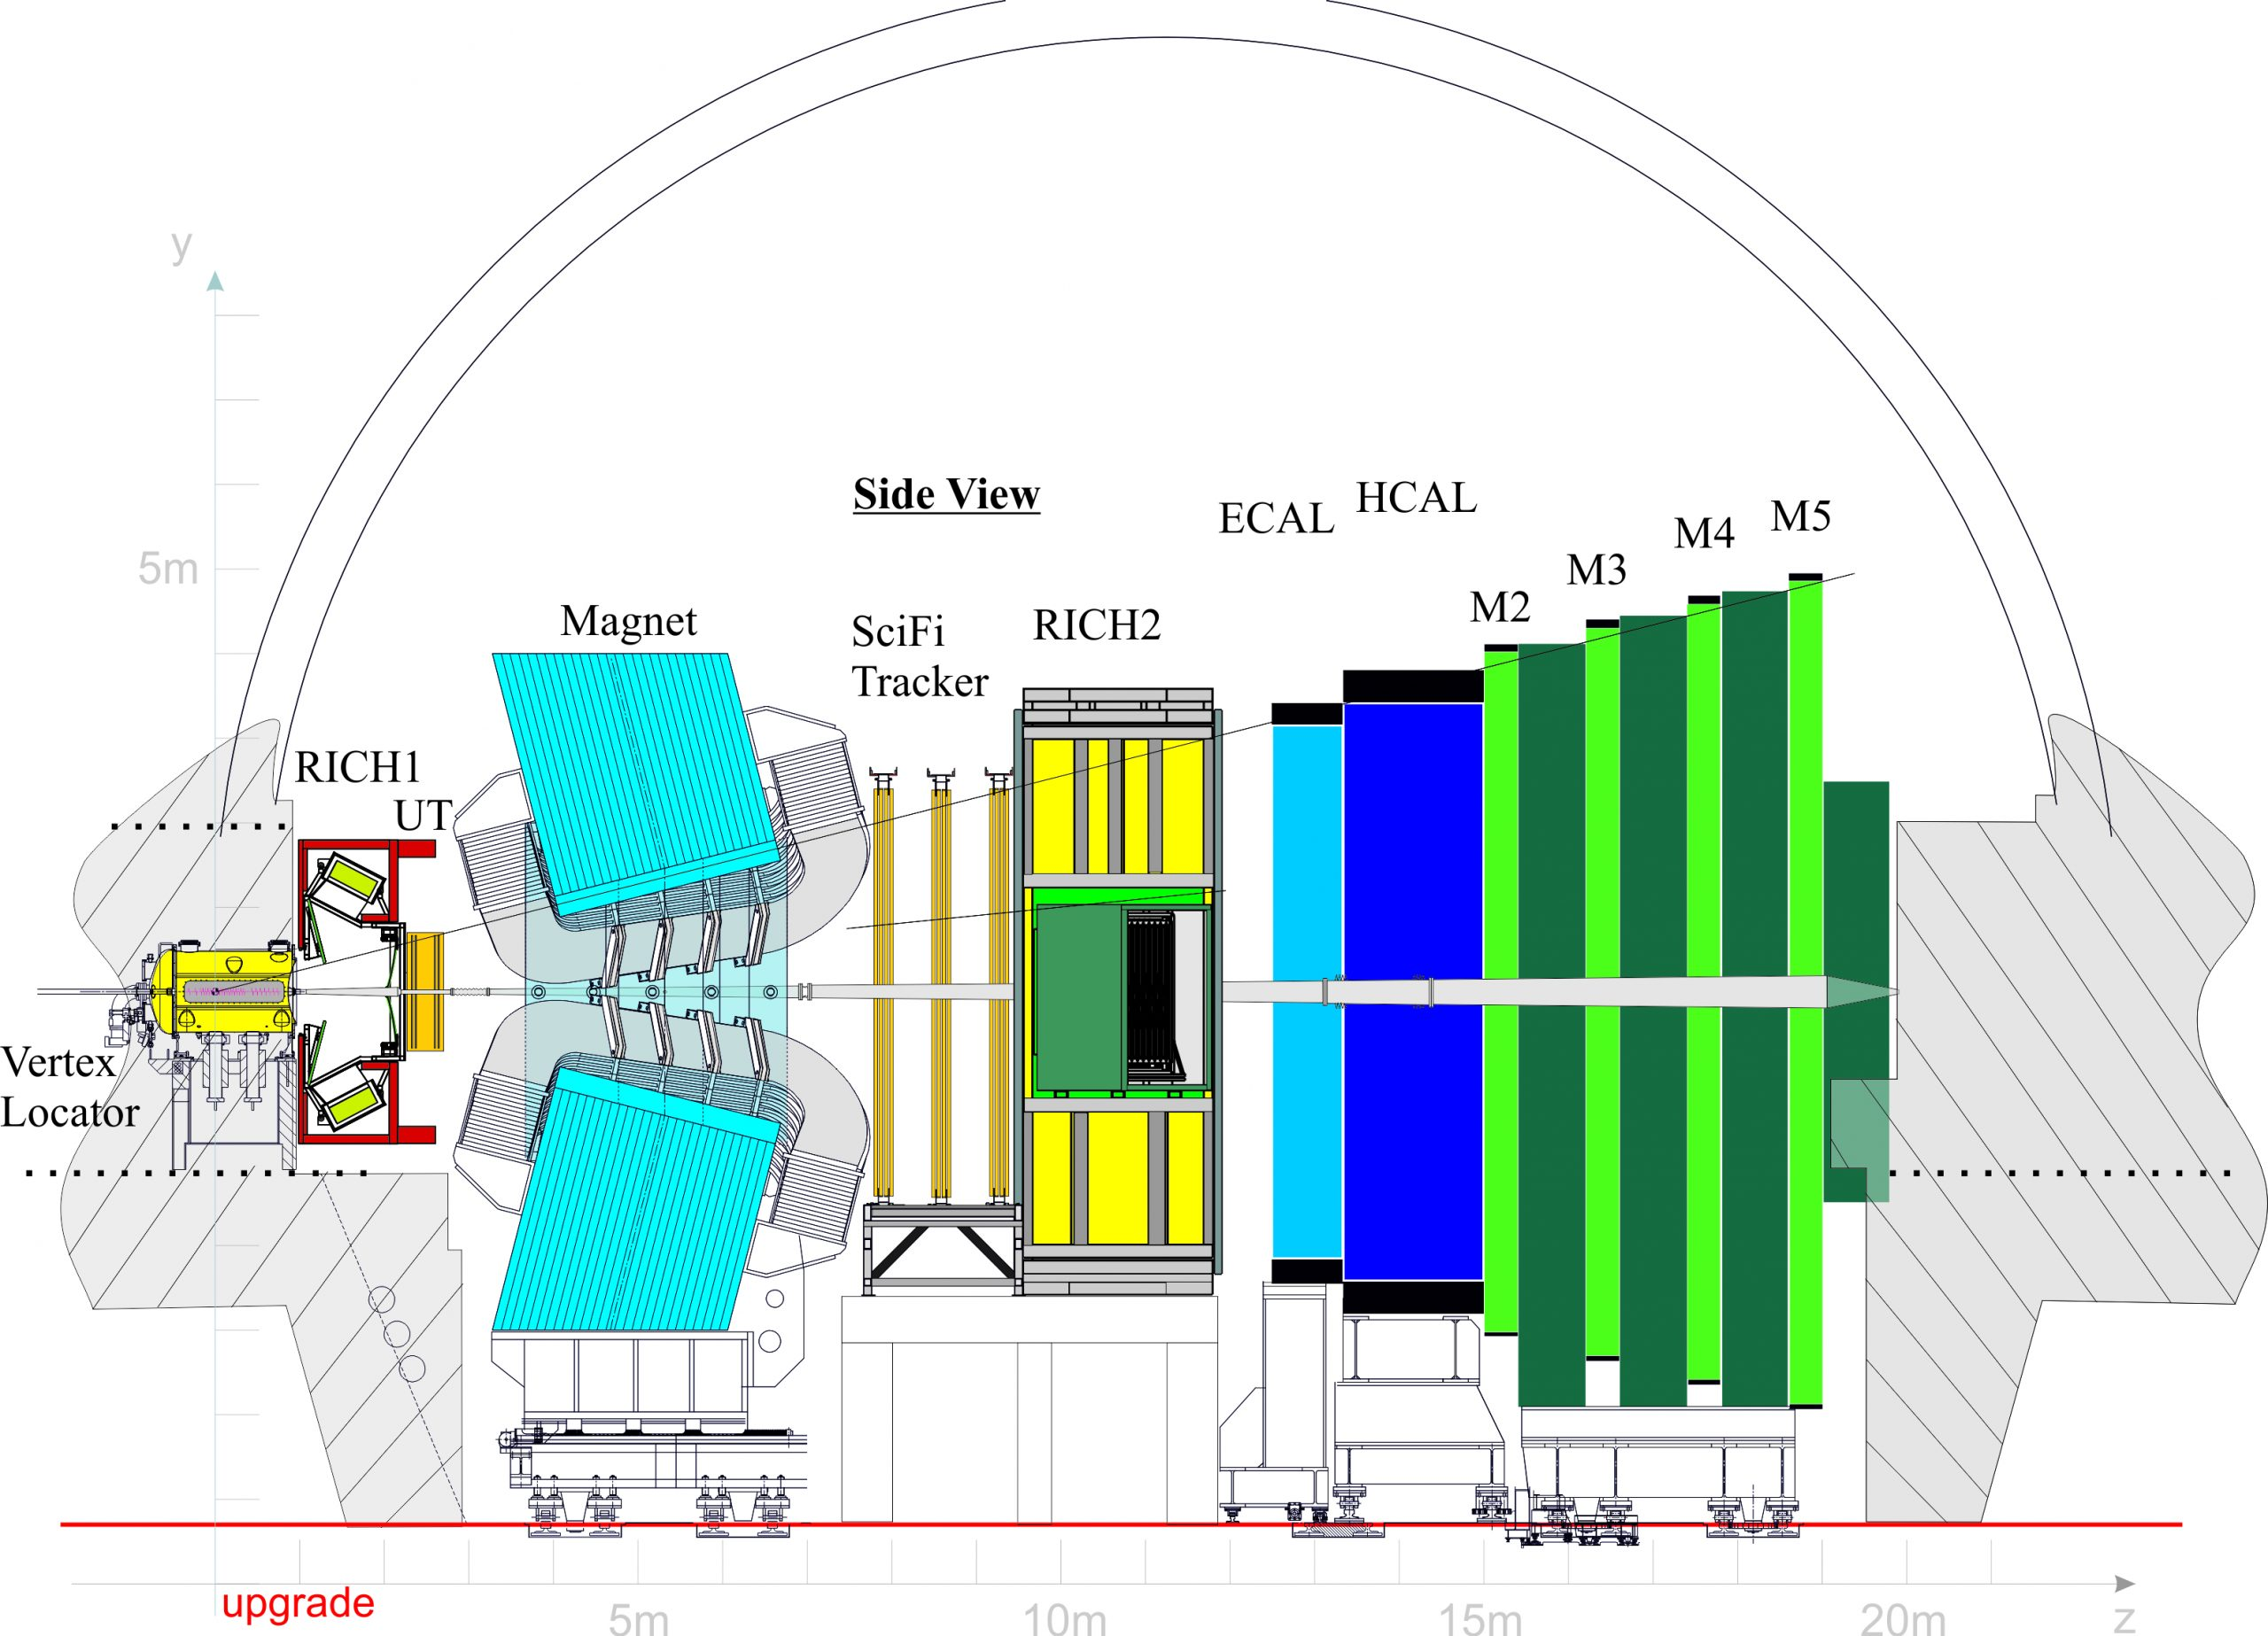
\includegraphics[width=\textwidth]{content/Figures/LHCb.jpg}
	\caption[Schematic view of the LHCb Upgrade 2 detector.]{Schematic view of a cross section of the LHCb Upgrade 1 detector \cite{TDR}.}
	\label{fig:LHCb}
\end{figure}
The LHCb detector is constructed as a single-arm forward spectrometer,
because the $b$-$\bar{b}$ pairs in $pp$ collisions are mainly produced at a small angle relative to the beam axis.
Therefore, the resulting hadrons are boosted in the same direction \cite{bbangles}.

In Figure \ref{fig:LHCb}, the cross section of the LHCb detector is shown.
The \textit{Vertex Locator} (VELO) is used to identify and distinguish the primary and secondary vertices of the particles.
Since these are only a few millimetres apart,
the VELO is located directly around the interaction point.
Together with the \textit{Upstream Tracker} (UT),
the \textit{dipole magnet} and the \textit{SciFi detector}, the VELO forms the spectrometer system of LHCb.
This system is used to reconstruct particle tracks and to determine the momentum,
which can be obtained from the deflection of the particles in a magnetic field.

The detectors \textit{RICH1}, \textit{RICH2}, \textit{ECAL}, \textit{HCAL} and the muon stations \textit{M2} to \textit{M5} are used for particle identification.
The focus here is on distinguishing electrons, photons, kaons and protons,
because they are common decay products of $b$ hadrons \cite{TDR}.
The RICH detectors are used to keep charged hadrons apart, especially pions, kaons and protons.
They measure the Cherenkov light emitted by charged particles and combine this information with the measured momentum of the track. This allows LHCb to assign a particle hypothesis to each reconstructed track.
This is essential for B decay analyses, because the final state particles must be identified correctly.
In the decay $\text{B}^+ \to K^+K^-K^+$, for example, all three charged tracks have to be identified as kaons.
A wrong particle identification would lead to a wrong reconstructed invariant mass. This leads to the background of the selected signal.\\
The calorimeters identify photons, electrons and hadrons, while the muon stations identify muons.
Together with the tracking system, these detectors allow the full reconstruction and classification of the decay products of $b$ hadrons.
\subsection{$\text{B}^{+/-}$ Mesons in the LHCb}
\label{sec:decay}
The B mesons are created in the primary vertex, which is the location of the collision of the proton beams. After a few pikoseconds some of these mesons decay into three Kaons. The decay looks like
\begin{equation*}
  \text{B}^+ \to K^+ \, K^- \, K^+
\end{equation*}
and for the anti-particle
\begin{equation*}
  \text{B}^- \to K^- \, K^+ \, K^-
\end{equation*}
with the quark-level Feynman diagram shown in \autoref{fig:bkkk}.\\\\
\begin{figure}[htbp]
\centering
\begin{tikzpicture}
\begin{feynman}

% Anfangszustand B+
\vertex (u_in)    at (0, 2.0) {$u$};
\vertex (bbar_in) at (0, 0.0) {$\bar b$};

% B+ Label links zwischen den Linien
\node at (-0.9, 1.0) {$B^+$};

% Vertices der unteren Linie
\vertex[dot] (v1) at (2.5, 0.0) {};
\vertex[dot] (v2) at (6.5, 0.0) {};

% Cut liegt zwischen v1 und v2
\vertex (u_cut_left)  at (4.2, 2.0) {};
\vertex (u_cut_right) at (4.8, 2.0) {};
\vertex (u_out)       at (10, 2.0) {$u$};

\vertex (cbar_cut_left)  at (4.2, 0.0) {};
\vertex (cbar_cut_right) at (4.8, 0.0) {};
\vertex (sbar_out_main)  at (10, 0.0) {$\bar s$};

% Labels mittig in der Lücke
\node at (4.5, 2.0) {$u$};
\node at (4.5, 0.0) {$\bar c$};

% Erster W+ Zweig: W+ -> u + sbar
\vertex[dot] (wplus) at (3.8, -1.6) {};
\vertex (u1)          at (5.8, -0.8) {$u$};
\vertex (sbar1)       at (5.8, -2.4) {$\bar s$};

% Zweiter W- Zweig: W- -> s + ubar
\vertex[dot] (wminus) at (7.8, -1.6) {};
\vertex (s2)          at (9.8, -0.8) {$s$};
\vertex (ubar2)       at (9.8, -2.4) {$\bar u$};

\diagram*{
  % Spectator-Linie mit Cut zwischen den W-Zweigen
  (u_in) -- [fermion] (u_cut_left),
  (u_cut_right) -- [fermion] (u_out),

  % Untere Quarklinie mit Cut zwischen den W-Zweigen
  (bbar_in) -- [anti fermion] (v1)
             -- [anti fermion] (cbar_cut_left),
  (cbar_cut_right) -- [anti fermion] (v2)
                   -- [anti fermion] (sbar_out_main),

  % Erster Zerfall: bbar -> cbar + W+
  (v1) -- [boson, edge label'=$W^+$] (wplus),
  (wplus) -- [fermion] (u1),
  (wplus) -- [anti fermion] (sbar1),

  % Zweiter Zerfall: cbar -> sbar + W-
  (v2) -- [boson, edge label=$W^-$] (wminus),
  (wminus) -- [fermion] (s2),
  (wminus) -- [anti fermion] (ubar2),
};

% Hadron-Labels
\node at (10.8, 1.0) {$K^+$};
\node at (6.3, -1.6) {$K^+$};
\node at (10.4, -1.6) {$K^-$};

\end{feynman}
\end{tikzpicture}
\caption{Quark-level diagram for $B^+ \to K^+K^-K^+$.}
\label{fig:bkkk}
\end{figure}
Kaons can also be produced directly at the primary vertex as relatively light particles in the proton-proton collision. To identify kaons originating from a secondary vertex, their tracks are reconstructed using the detector hits and their deflection in the magnetic field. From the reconstructed track, the distance of closest approach to the primary vertex can be determined. This distance is called the \textit{impact parameter}. If the impact parameter is small, the tracked particle is likely to originate from the primary vertex. If the impact parameter is large, the particle is more likely to originate from a secondary vertex.\\\\
CP violation can be observed in decays of $B$ mesons, because these mesons contain a $b$ quark or a $\bar b$ quark. The $b$ quark decays via the weak interaction. In the Standard Model, the weak transitions between different quark flavours are described by the CKM matrix. This matrix contains a complex phase, which is the source of CP violation.\\
In the Wolfenstein parametrisation, the CKM matrix can be written as
\begin{equation*}
V_{\mathrm{CKM}} \approx
\begin{pmatrix}
1 & \lambda & A\lambda^3(\rho - i\eta) \\
-\lambda & 1 & A\lambda^2 \\
A\lambda^3(1-\rho-i\eta) & -A\lambda^2 & 1
\end{pmatrix}.
\end{equation*}
Here, $\lambda = \sin{\Theta_C} \approx 0.22$ is a small parameter. The terms containing $i\eta$ make the matrix complex. Therefore, the decay amplitudes of a particle and its antiparticle can be different.\\
In $B$ meson decays, different decay paths can lead to the same final state with different CKM factors. The interference can lead to different decay rates for $B^+$ and $B^-$. This results in a CP asymmetry. There is a global and a local asymmetry. The global asymmetry compares the total number of $B^+$ and $B^-$ decays. The CP violation can be stronger in some regions of the phase space than in others. This local behaviour can be investigated with Dalitz plots, which are discussed in \autoref{sec:dalitz}.
\subsection{Dalitz-plots}
\label{sec:dalitz}
Dalitz plots are used to describe three-body decays. For each event, two invariant masses of two-particle combinations are calculated and plotted against each other. In this way, each reconstructed decay gives one point in the Dalitz plot. Therefore, Dalitz plots are used to study local CP asymmetries.

For the $\text{B}^{+/-}$-decay the variables are set to
%%%%%%%%%%%%%%%%%%%%%%%%%%%%%%%%%%%%%%%%%%%%%%%%%%%
\begin{equation*}
m^2(m_1 m_2)
\end{equation*}
and
\begin{equation*}
m^2(m_1 m_3).
\end{equation*}
%%%%%%%%%%%%%%%%%%%%%%%%%%%%%%%%%%%%%%%%%%%%%%%%%%%
The B meson can decay over an intermediate resonance. For example, the decay
\begin{equation*}
B^+ \to K^+ K^- K^+
\end{equation*}
can proceed through an intermediate resonance $R$
\begin{equation*}
B^+ \to K^+ R, \qquad R \to K^- K^+ .
\end{equation*}
For the charge-conjugated decay this becomes
\begin{equation*}
B^- \to K^- R, \qquad R \to K^+ K^- .
\end{equation*}
Intermediate resonances are shown as bands in the Dalitz plot. Many events are found around the resonance mass because the intermediate resonance is produced with a higher probability when the invariant mass of the two-particle system is close to its mass. The events are spread over a small mass region and form a band.
